\documentclass{article}
\usepackage[utf8]{inputenc}
\usepackage{mathtools}
\usepackage{todonotes}
\usepackage{amsmath}
\usepackage[ruled,vlined]{algorithm2e}
\usepackage{amssymb}
\usepackage[hidelinks]{hyperref}
\usepackage{caption}
\usepackage{placeins}
\usepackage{subcaption}
\usepackage{siunitx}
\usepackage{mathrsfs}
\usepackage{xcolor}
\usepackage[citestyle=alphabetic,bibstyle=numeric]{biblatex}
\usepackage{float}
\usepackage{booktabs}
\usepackage{xcolor}
\usepackage{xparse}
\usepackage{graphicx}



\newlength\tindent
\setlength{\tindent}{\parindent}
\setlength{\parindent}{0pt}
\renewcommand{\indent}{\hspace*{\tindent}}

\newcommand{\RNum}[1]{\uppercase\expandafter{\romannumeral #1\relax}}

\NewDocumentCommand{\codeword}{v}{%
\texttt{\textcolor{gray}{#1}}%
}


\addbibresource{bibliography.bib}

\title{DeepVision - Deep Learning and Convolutional Neural Networks in Computational Vision:\\
Group Normalization Project}
\author{Marco Deuscher \\\href{mailto:marco.deuscher@uni-ulm.de}{marco.deuscher@uni-ulm.de}}
\date{Summer Term 2021}

\begin{document}
    \maketitle

    \section{Introduction}\label{sec:introduction}
For many applications, high resolution inputs and outputs are required, such tasks include semantic segmentation, instance segmentation, depth estimation or visual generative models.
Here the amount of memory that is required during the training process surmounts the available memory on many consumer GPUs.
Thus, training such models is often conducted on multiple GPUs in a synchronized manner.
This however poses a limitation if the amount of computational power, especially memory is limited and only a single graphics card is available during training.
One possible solution for such a scenario is training on a lower resolution, however this often negatively impacts the performance of the model.
Thus, the need to develop an effective normalization procedure that is independent of the batch size arises.
The commonly employed Batch Normalization layer introduces larger error for smaller batch sizes as the estimation of the batch statistics become faulty.
Such an idea is presented in the Group Normalization paper by Wu and He~\cite{DBLP:journals/corr/abs-1803-08494}.
    \section{Reading and Theory}\label{sec:reading-and-theory}
The following firstly revises the basic idea presented in the paper and presents its main conclusions.
Secondly, the contents of the paper are discussed in the context of the Lecture Deep Vision - Deep Learning and Convolutional Neural Networks in Computational Vision and the position of the paper in the literature is discussed.
Lastly, remaining issues and suggestions for future work are presented.

\subsection{Revision of the Content}
Batch normalization is used in many network architectures as it offers faster training due to the distribution being closer to the initial initialization of the weights by normalizing each batch to zero mean and unit variance.
Further, the normalization creates a small error due to the running mean and variance that acts as a regularization similar to the addition of noise.
However, there are some drawbacks to the usage of batch normalization.
The statistics (mean and variance) are computed during training and are kept during inference, hence if the distribution changes the normalization is not valid anymore.
Another issue is the aforementioned problem of larger statistical errors when using smaller batch sizes.
So there is the need for a normalization technique which is independent of the batch size.
There are layer norm and instance norm which normalize all channels and single channels respectively.
However, they have been shown to not work as well for visual tasks.
The in the paper presented group normalization partitions the channels in individual groups that are then normalized separately.
The idea to group channels is motivated by many classical computer vision features where some form of group normalization is applied.
This is especially true for the first layers in a network where orientation sensitive filters may result in similar distributions and may thus be normalized together.
For higher level features this is less intuitive but there may still exist a dependency between individual feature channels.
Furthermore, the idea to group channels has been exploited in other contexts as well.
One well known example is the ResNext architecture~\cite{DBLP:journals/corr/XieGDTH16} where in each residual block the channels are grouped into smaller convolutions, outperforming the original ResNets on the ImageNet challenge.\\

The original batch normalization layer normalizes along the $(N, H, W)$ axes, where $N$ is the batch size.
Hence, there is a obvious dependence on the batch size and it is clear why the statistical error increases when the batch size decreases.
Instance normalization computes the mean and variance separately for each sample in the batch and each channel,
layer normalization computes the mean and variance for each sample but includes all channels and spatial resolution.
Thus, instance and layer normalization have no dependence on the batch size in their computation.
Group norm splits the channels into groups with a group size that is specified by an additional hyperparamter.
Group normalization then computes the mean and variance for each group and each sample, making it independent of the batch size as well.\\

In the paper they evaluated the performance of the different normalization layers firstly on the ImageNet classification dataset.
A ResNet-50 was trained on the batch sizes $\{32, 16, 8, 4, 2\}$, the results clearly show that for the larger batch sizes ($32, 16$) the group norm layer is only slightly outperformed by the batch norm whereas for the smaller
batch sizes ($4,2$) the group norm is able to significantly outperform the batch normalization layer.
It is observed that the group normalization is robust as the performance does not deteriorate for larger batch sizes.
This behaviour is later reproduced in section~\ref{sec:implementation}.\\
They further experimented with the group normalization layer by integrating them into the Mask R-CNNs and training them on COCO for the task of object detection.
Again they were able to show group normalization outperforming the previously employed batch normalization.\\
Lastly, they evaluated the behaviour on a video classification task where the normalization layers were extended to include tne temporal axis.
Group normalization again showed a similar performance for the larger batch size of 8 and outperformed batch normalization for the smaller batch size of 4.

\subsection{Context of the Paper}
The context of the paper in the literature is one in which a new normalization technique is proposed that enables researches to experiment with the usage in different network architectures and potentially find architectures better suited to this specific form of normalization.
In the context of the lecture Deep Vision group normalization relates to the concepts covered in chapter \RNum{4} Training Deep Network Architectures.
After quickly motivating the need for normalization in deep networks two main techniques are discussed.
Firstly, Local Response Normalization (LRN) where neighboring channels at a single position or local spatial neighborhoods are normalized together.
Secondly, the previously discussed techniques of batch, layer, instance and group normalization.
The paper primarily relates to the second technique, hence LRN is not discussed any further in the following.
The internal covariance shift describes the phenomenon that the distribution may change in a deep network, to prevent this from happening normalization layers are applied at various stages of a network to renormalize the activations to zero mean and unit variance.
The lecture quickly covers the aforementioned batch normalization algorithm and points out the potential problem when training with small batch sizes.
Furthermore, the layer norm, instance norm and group norm algorithms are discussed and as in the original paper the relationship between the different normalization techniques is mentioned.
Meaning that group normalization and layer normalization are identical if the number of channels per group is set to one.
Similarly, group normalization and instance normalization are identical when the group number is set to the number of channels in the individual layer.\\

Taking a step back, the presented normalization techniques relate to techniques or concepts to stabilize and improve the training of deep networks.
Other techniques for this that were mentioned during the lecture are advanced optimizers such as Adam, weight initialization techniques to minimize the required learning by the netowrk
but also regularization techniques such as dropout and data augmentation.
Also mentioned in this context were techniques on a systems level such as fine-tuning and transfer-learning where entire parts of a network are utilized that were previously trained for a different task, for visual tasks this is commonly the ImageNet classification task.
Other similar techniques include unsupervised pretraining, e.g. as an autoencoder to learn useful representations.

\subsection{Future Work}
Due to this paper introducing a novel concept for normalization which is independent of the batch size but appears to work better for visual tasks much of the future work is integrating it into established architectures to test its performance.
Further, to apply this concept to current research to possibly find network architectures that natively incorporate group normalization layers.
One of the aspects mentioned in the paper is the application of group normalization in generative models as they have a significant memory footprint.
    \section{Implementation}\label{sec:implementation}
For the replication of the results presented in section~\ref{sec:reading-and-theory} I decided to use pytorch\footnote[1]{\href{https://pytorch.org/}{https://pytorch.org/}} due to personal preference and previous experience.
The implementation consists of a library which can be found in the \codeword{src} folder.
The library contains the implementation of all models, datasets, training and evaluation methods.
Further, a notebook is provided in the root directory, offering access to the implemented library functions and using them for training, evaluation and visualisation.
In the following firstly the two implemented datasets CIFAR-10 and FashionMNIST are introduced in section~\ref{subsec:datasets}, then the implemented models and their respective architecture is presented in section~\ref{subsec:models}.
Section \ref{subsec:training} describes the training process.
Finally, the results achieved by the models are discussed in section~\ref{subsec:evaluation}.

\subsection{Datasets}\label{subsec:datasets}
The following introduces the CIFAR-10 and FashionMNIST dataset.

\subsubsection{CIFAR-10}
The CIFAR-10~\cite{CIFAR10} is a dataset for the task of classification consisting of a total of 60.000 images from 10 different classes including various vehicles and animals.
The individual images have a size of $32\times 32$ and are given as RGB images.
The training split contains 50.000 images and the test split the remaining 10.000.
As my exploration of the hyperparameter space is extremely limited I decided against using an additional validation split as it is highly unlikely for the hyperparameters to overfit.

\subsection{FashionMNIST}
The FashionMNIST~\cite{DBLP:journals/corr/abs-1708-07747} dataset is a dataset for the task of classification dataset inspired by the original MNIST dataset which contains handwritten digits.
The dataset consists of 10 classes each representing a fashion item.
FashionMNIST contains a total of 60.000 training images and an additional 10.000 test images.
Again, I decided not to use a validation split.
The images are given as $28\times 28$ gray-scale images.
Figure~\ref{fig:datasets_ex} shows three examples from both of the datasets.
\begin{figure}[t]
    \centering
    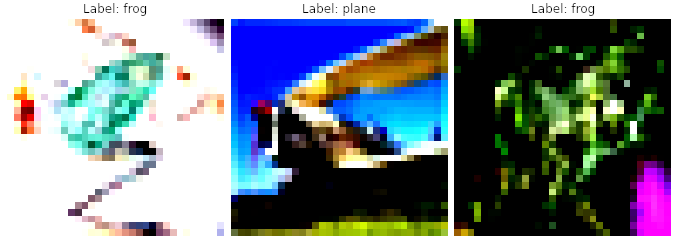
\includegraphics[width=.45\textwidth]{res/CIFAR.png}
    
\includegraphics[width=.45\textwidth]{res/MNIST.png}
    \caption{Three examples from the CIFAR-10 dataset with their respective labels on the left and the MNIST dataset on the right.}
    \label{fig:datasets_ex}
\end{figure}

\subsection{Models}\label{subsec:models}
The models implemented in \codeword{src/models} contain a ResNet-34~\cite{he2015deep}, a implementation of the GroupNorm layer and two simple CNNs SimpleNet and SimpleNetv2.
My implementation of the GroupNorm utilizes the code provided in the original paper~\cite{DBLP:journals/corr/abs-1803-08494} and wrapped it inside a module for the convenient management of parameters.
For the ResNet the basic residual block proposed in~\cite{he2015deep} and the ResNet-34 architecture is used.
I tried using a ResNet as it is a well established architecture achieving good results on many tasks, however I was unable to train the smaller batch sizes using ResNet as the time required for training was not feasible for me.
However, I decided to use the results of the ResNet-34 as baseline to compare to other models.\\
The SimpleNetv2 consists of three SimpleBlocks, their architecture is shown in figure~\ref{fig:simplenet} on the left.
The SimpleBlock contains two stacked convolutions.
After the first convolution, the number of input channels is doubled.
After each convolution a normalization layer and ReLU are applied.
Finally, each SimpleBlock is terminated by a Max-Pooling operation, reducing the spatial resolution by a factor of two.
The full architecture of the SimpleNetv2 is shown in figure~\ref{fig:simplenet} on the right.
The first basic block increases the number of channels from 3 to 32.
The three basic blocks achieve an output stride of 8.
Finally, two linear layers using ReLU and no activation respectively, with the first one having 1024 neurons and the output having 10 neurons.
\begin{figure}[h]
    \centering
    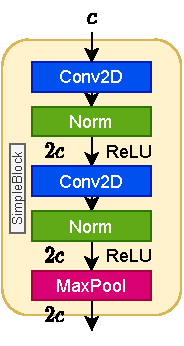
\includegraphics[width=.3\textwidth]{res/basicBlock.pdf}
    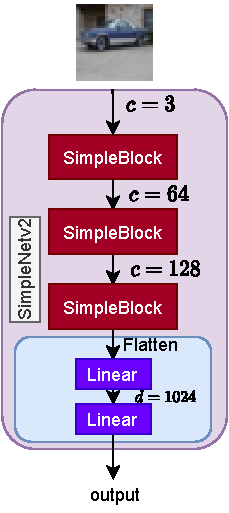
\includegraphics[width=.25\textwidth]{res/SimpleNetv2.pdf}
    \caption{Architecture of the simple basic block on the left and the SimpleNetv2 on the right.}
    \label{fig:simplenet}
\end{figure}

\subsection{Training}\label{subsec:training}
The training procedure described in the following is used for both the CIFAR-10 model and the FashionMNIST model.
However, the evaluation solely considers the CIFAR-10 dataset.
The training was conducted on a Nvidia GTX 1660ti with 6GB of VRAM.
As a loss function a standard cross-entropy loss is utilized.
For optimization an Adam optimizer with weight decay was employed with the following parameters $\text{lr}=0.001, \beta_1=0.9, \beta_2=0.999, \varepsilon=1\cdot 10^{-8}$ and for the weight decay $\lambda=0.01$.
I experimented with different optimizers including Adam without weight decay and SGD but the above named configuration was the most stable and achieved the best results.
Furthermore, a cosine annealing learning rate scheduler is used.
The SimpleNetv2 network was trained for a total of 30 epochs, whereas the ResNet-34 was trained for a total of 200 epochs on the dataset.
During training the following batch sizes are used $\{2, 4, 8, 16, 32, 64\}$.
The models employing group normalization are trained using a group size of 16.

\subsection{Evaluation}\label{subsec:evaluation}
After training a total of thirteen networks on the CIFAR-10 dataset using the training procedure described above the following results are obtained.
\begin{figure}[h]
    \centering
    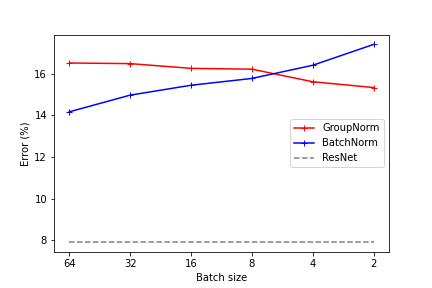
\includegraphics[width=.85\textwidth]{res/plot.png}
    \caption{Evaluation}
    \label{fig:eval}
\end{figure}
Figure~\ref{fig:eval} displays the achieved results.
The x-Axis marks the different batch sizes, the y-Axis the error of the model on the test split.
The result of the best ResNet-34 is shown as the dashed gray line and is used as a baseline.
The batch norm and the group norm are shown in blue and red respectively.
The figure clearly shows that the model using batch norm drastically improves when the batch size increases.
Further, the group norm degrades with a higher batch size but not nearly as bad as the batch norm.
However, this behaviour is not intuitive as the batch size should not directly affect the group normalization.
For small batch sizes (e.g. 2 and 4) the group norm models are able to outperform the batch norm models.
For larger batches sizes (batch size $> 4$) the batch norm model starts to outperform the group norm.
Compared to the results obtained in the original paper the difference between batch and group norm for small batch sizes is significantly smaller.
My explanation for this behaviour is that this is due to the dataset.
Compared to ImageNet, CIFAR-10 is a significantly easier dataset on which a less complex model is still able to achieve a good performance.
This idea is supported by the fact that the difference between batch and group norm on the FasionMNIST dataset is even smaller.
During my evaluation of the FashionMNIST dataset all models were within $1.5\%$ but the order was still as expected, meaning for batch size 2 the group norm outperformed the batch norm.
Furthermore, during my experiments with the ResNet-34 on CIFAR-10 the difference between group and batch norm appeared to be similar to the results achieved by the SimpleNetv2.
However, I do not have an explanation for the deterioration of the group norm for larger batch sizes.

    \section{Conclusion}\label{sec:conclusion}
The goal of this report was the reproduction of the results the original paper presented.
This was partly achieved as presented in section~\ref{subsec:evaluation}.
For smaller batch sizes the expected behaviour of group norm was achieved whereas for larger batch sizes the performance deteriorated unexpectedly.
However, the main use case for employing group normalization are models with a large memory footprint which certainly was not the case for the used model.
During my bachelor thesis on Depth Estimation using CNNs I experimented with the usage of group normalization as training was conducted on a single GPU.
However, I was unable to adapt the model such that I would achieve similar performance when using group normalization.
For many other tasks including the tasks evaluated in the paper, group normalization offers the possibility of training with a significantly smaller batch size that enables researches to experiment with higher capacity models.





    \printbibliography

\end{document}
